\subsection{Product perspective}
\subsubsection{Scenarios}

\comment{Sono da scrivere per esteso sotto forma di esempio, solo una traccia per ora}

\begin{enumerate}
   \item Creating a Tournament:
        \begin{itemize}
            \item Educator logs in to the CKB platform;
            \item Educator creates a new tournament;
            \item Educator sets tournament details, including a description, start and end dates, and any specific rules;
            \item CKB notifies all subscribed students about the new tournament.
        \end{itemize}

   \item Creating a Code Kata Battle:
        \begin{itemize}
            \item Educator selects a tournament to create a code kata battle within;
            \item Educator uploads the code kata, including the description, software project, and build automation scripts;
            \item Educator sets the minimum and maximum number of students per group, registration deadline, final submission deadline, and additional scoring configurations;
            \item CKB platform notifies all subscribed students about the new battle.
        \end{itemize}

    \item Student partecipates to a Battle:
        \begin{itemize}
            \item Students log in to the CKB platform;
            \item Students join a code kata battle individually or invite others to form a team;
            \item Students adhere to the minimum and maximum number of students per group set for the battle.
            \item Students fork the GitHub repository and set up automated workflows using GitHub Actions;
            \item Students commit code changes to the main branch;
            \item CKB platform is triggered on each push, pulling the latest sources and running tests to calculate and update the team's score.
            \item Scores are updated in real-time on the platform, visible to both students and educators.
        \end{itemize}

    \item Educator manually evaluates Students' solutions:
        \begin{itemize}
            \item After the submission deadline, there is a consolidation stage;
            \item CKB platform automatically evaluates functional aspects, timeliness, and source code quality;
            \item Educator may manually evaluate and assign a personal score;
            \item If manual evaluation is required, the educator reviews and scores the sources produced by each team;
        \end{itemize}

    \item Tournament Closure and Notifications:
        \begin{itemize}
            \item Educator closes the tournament;
            \item CKB platform notifies all students involved in the tournament;
            \item Personal tournament scores are updated for each student.
        \end{itemize}

    \item Gamification Badges:
        \begin{itemize}
            \item Educator creates gamification badges for the tournament;
            \item Badges have titles and rules based on predefined variables;
            \item Students earn badges based on their performance in battles.
            \item Badges are displayed with their titles and associated rules;
        \end{itemize}
    
\end{enumerate}

\subsubsection{Domain class diagram}
\comment{Descrizione del class diagram}

\begin{figure}[h!]
  \centering
  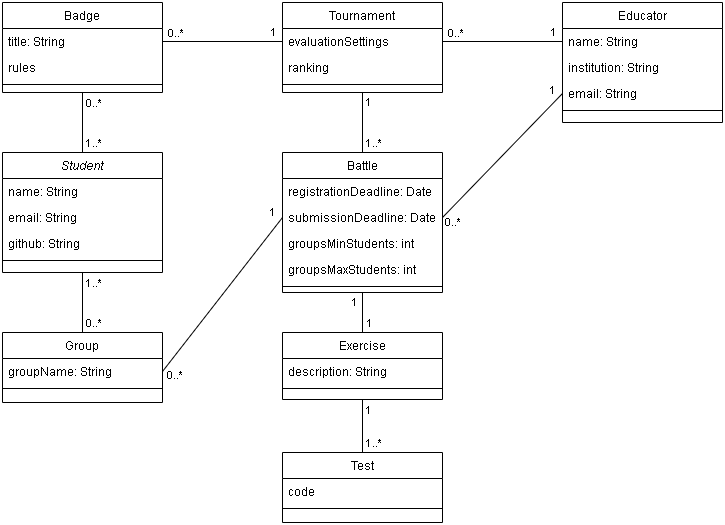
\includegraphics[width=0.8\textwidth]{Images/ClassDiagramRASD.png}
  \caption{Domain class diagram}
  \label{fig:ClassDiagram}
\end{figure}

\subsubsection{Statecharts}

\comment{Fare i diagrammi}

The CKB platform involves several key states and transitions to facilitate the seamless execution of code kata battles and tournaments. The primary states and transitions are described below:

\begin{enumerate}
    \item Tournament Lifecycle:
        \begin{itemize}
            \item States: Registration, Started, Closed
            \item Transitions: from Registration to Started (triggered when an educator starts a new tournament) and from Started to Closed (triggered when an educator decides to close the tournament)
        \end{itemize}

    \item Code Kata Battle Lifecycle:
        \begin{itemize}
            \item States: Created, Registration, Started, Consolidation, Closed
            \item Transitions: From Created to Registration Open (triggered when an educator creates a new code kata battle), From Registration Open to Started (occurs after the specified registration deadline), Started to Consolidation (when the battle ends, if required), Consolidation to Closed (when the evaluation ends)
        \end{itemize}

    \item Student Team Formation:
        \begin{itemize}
            \item States: Pending, Accepted, Rejected
            \item Transitions: From Pending to Accepted (occurs if the number of teammates that joined the group by accepting the invitation is within the range) of from Pending to Rejected (occurs when the number of teammates that accepted the invitation is lower than the minimum number, either at the end of the registration phase or after other students decline the invitation)
        \end{itemize}

    \item GitHub Integration:
        \begin{itemize}
            \item States: Repository Created, Workflow Established, Battle Closed
            \item Transitions: From Repository Created to Workflow Established (Students fork the GitHub repository and configure automated workflows) and Workflow Established to Battle Closed (Triggered when the battle's deadline expires)
        \end{itemize}

    \item Battle Score Update:
        \begin{itemize}
            \item States: Real-time Update, Consolidation Stage, Final Score
            \item Transitions: From Real-time Update to Consolidation Stage (Triggered after the submission deadline, indicating a transition to manual evaluation if necessary), from Consolidation Stage to Final Score (when the educator ends the manual evaluation).
        \end{itemize}

    
\end{enumerate}

\subsection{Product functions}

\comment{sostituire subsubsection con lista}

\subsubsection{Tournament Management}
 \begin{itemize}
    \item Create Tournament: educators can create new tournaments, specifying details such as description, start and end dates, and rules.
    \item Close Tournament: educators have the ability to close a tournament, signaling the end of the competition.
    \item Add Battles: educators can add battle to their tournaments or allows other educators to add them.
\end{itemize}

\subsubsection{Code Kata Battle Management}
 \begin{itemize}
    \item Create Code Kata Battle: educators can create code kata battles within a tournament, providing details such as the kata description, software project, build scripts, and scoring configurations.
    \item Set Battle Deadlines: educators can set registration and submission deadlines for each code kata battle.
\end{itemize}

\subsubsection{Student Interaction}
\begin{itemize}
    \item Registration and Team Formation: students can register for individual battles or form teams based on the specified team size limits. Teams are formed before the registration deadline.
\end{itemize}

\subsubsection{GitHub Integration}
\begin{itemize}
    \item Repository Creation: after the registration deadline, the platform automatically creates a GitHub repository for each team.
    \item Automated Workflow: students set up automated workflows using GitHub Actions to enable continuous integration. CI processes are triggered with each commit, updating the CKB platform in real-time.
\end{itemize}

\subsubsection{Scoring evaluation}
\begin{itemize}
    \item Automated Scoring: the platform automatically evaluates functional aspects, timeliness, and source code quality.
    \item Real-time Score Updates: scores are updated in real-time on the platform, visible to both students and educators.
    \item Manual Evaluation: educators can manually evaluate and assign personal scores, if required.
\end{itemize}

\subsubsection{Tournament Closure}
\begin{itemize}
    \item Close Tournament and Notify: educators can close a tournament, and the CKB platform notifies all students involved. Personal tournament scores are updated for each student.
\end{itemize}

\subsubsection{Gamification Badges}
\begin{itemize}
    \item Badge Creation: educators can create gamification badges associated with specific tournaments.
    \item  Badge Assignment: badges are automatically assigned based on predefined rules and student performance. Students and educators can view earned badges in a student's profile.
\end{itemize}

\subsubsection{Notification System}
\begin{itemize}
    \item Automatic Notifications: The platform automatically notifies students and educators about new tournaments, battles, and tournament closures. Notifications include important deadlines and updates.
\end{itemize}

\subsection{User characteristics}

\subsubsection{Educators}
\begin{itemize}
    \item Description: Educators play a crucial role in managing and overseeing the CKB platform. They are responsible for creating tournaments, defining code kata battles, and evaluating student submissions.
    \item Characteristics: Possess a deep understanding of software development concepts and practices. Have the authority to create, manage, and close tournaments. Able to assess student submissions based on various criteria, including code quality and adherence to coding practices.
\end{itemize}

\subsubsection{Students}
\begin{itemize}
    \item Description: Students are the primary users who participate in code kata battles and tournaments. They register for battles, form teams, and actively engage in coding exercises to demonstrate their software development skills.
    \item Characteristics: Have a basic understanding of programming languages and software development. Are motivated to improve their coding skills through practical challenges. Collaborate with team members during code kata battles to achieve common goals.
\end{itemize}


\subsection {Assumptions, dependencies and constraints}

\subsubsection{Assumptions}
\begin{itemize}
    \item The users (educators and students) have basic proficiency in using web-based platforms and are familiar with version control systems, such as Git.
    \item Educators have the necessary knowledge to create meaningful code kata battles, including defining test cases and scoring criteria
    \item Educators and students can connect to the Internet with their devices.
    \item Notification must arrive to connected users in one minute
    \item GitHub Account Requirement: students are required to have a GitHub account for participation, and the platform assumes that students have the necessary permissions to fork repositories.
    \item e-mail required
\end{itemize}

\subsubsection{Dependencies}
\begin{itemize}
    \item GitHub Integration: the CKB platform relies on GitHub for repository hosting and continuous integration processes.
    \item External APIs: Integration with external services may be required for additional functionalities, such as static code analysis tools.
    \item Internet Connectivity: Users (educators, students, administrators) need a reliable internet connection to interact with the CKB platform.
\end{itemize}

\subsubsection{Constraints}
\begin{itemize}
    \item Programming Languages: the platform supports a variety of programming languages for code kata battles, for example Java, Python, C, ...
    \item Browser Compatibility: the CKB platform is optimized for modern web browsers (e.g., Chrome, Firefox, Safari).
    \item Scalability: the platform must be designed to handle a scalable number of concurrent users during peak periods, such as registration deadlines.
     \item Security: the platform must adhere to security best practices to protect user data and prevent unauthorized access (sandboxing system since scripts can be malicious).
\end{itemize}